\documentclass{book}
\usepackage[utf8]{inputenc}

\title{Space Systems Lab Firmware and Mission Requirements Document}
\author{Hersch Nathan}
\date{November 2024}

\usepackage{url}
\usepackage{float}
\usepackage{natbib}
\usepackage{graphicx}
\usepackage{listings}
\usepackage{fullpage}
\usepackage{hyperref}
\hypersetup{
    colorlinks=true,
    linkcolor=blue,
    filecolor=magenta,      
    urlcolor=cyan,
}

\begin{document}

\maketitle

\section{General Requirements}
\par This software is to support the KRUPS missions. The current mission is KRUPS Aboard Norwegian GhostSat (KANGS). The hardware paradim is based around an ESP32-S3. 
\par This work is porting Matt Ruffner's firmware for Adafruit Feather M0/M4 to the ESP32-S3. This including switching from the Arduino IDE to ESP-IDF.
\par The goal of this project is to make the firmware more modular and configurable for each mission and hardware.
\par The first chapter of this document outlines the over all architechure design and background information for this project. The second chapter rt details each libraries, drives, wrappers, and other software components that we wrote for this project. It provides design decisions and the reasoning behind them aswell as how to interface with them. The third and on details the software requirements for each hardware component for each mission.

\tableofcontents

\chapter{Architechure Design} 
\section{Background Information}

\subsection{freeRTOS}
\par freeRTOS is a real time operating system. A real time operating system works by having tasks that run at different priorities. The tasks are scheduled by the operating system and those tasks occur through a determanistic prosess. The tasks can communicate with each other using message queues. The tasks can also synchronize with each other using semaphores.

\subsection{ESP-IDF}
\par ESP-IDF is the Espressif IoT Development Framework. It is the official development framework for the ESP32 and ESP32-S3. It is a set of libraries and tools that are used to develop software for the ESP32 and ESP32-S3.

\section{Overall Architecture Design}
\par The firmware's framework is designed to be modular and configerable thmission and each hardware. The backbone of the firmware is using freeRTOS tasks to handle the different modules. Each taks is its own module that encapsulates the relevant hardware. The tasks communicate with each other using a publisher/subscriber model.

\begin{figure} [H]
    \centering
    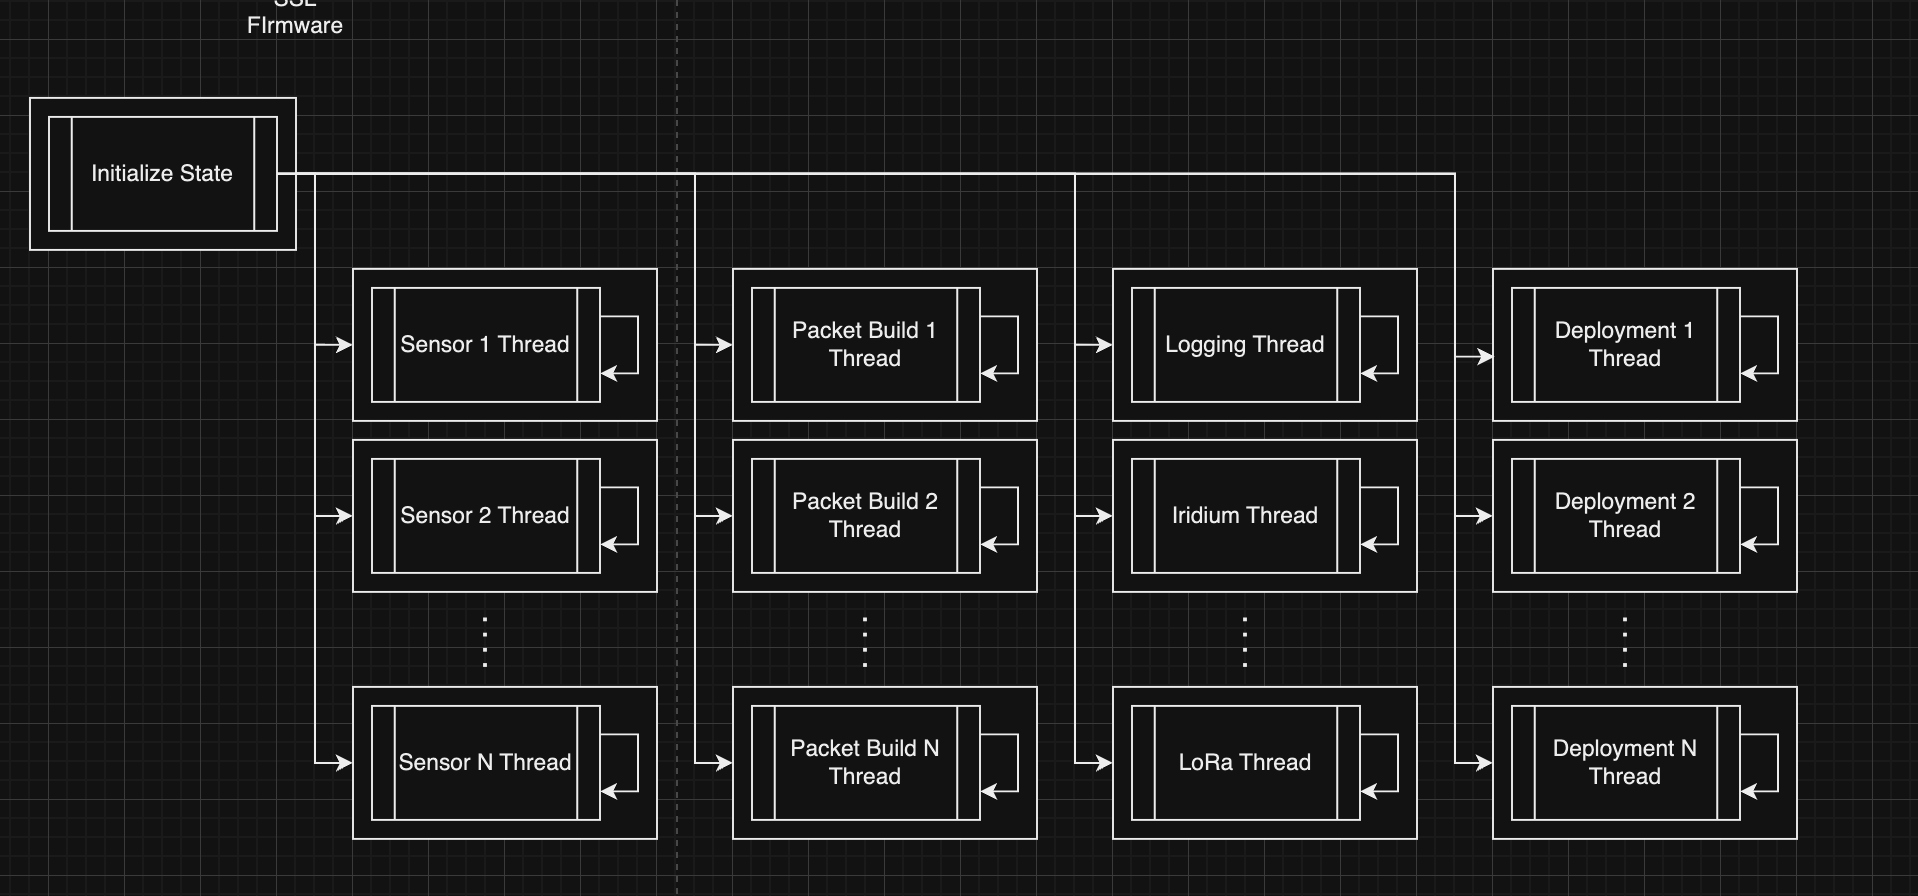
\includegraphics[width=0.8\textwidth]{images/firmware-architecture.png}
    \caption{Firmware Architecture}
    \label{fig:firmware-architecture} 
\end{figure}

\par In the figure \ref{fig:firmware-architecture}, the main tasks there are four types of tasks. 
\subsection{Task}
\subsubsection{Sensor Tasks}
\par Each sensor task manages one sensor or group of sensors, see \ref{fig:sensor-architecture}. At startup it configures the sensors with the necessary parameters, then it calls a looping task. That task, takes the semaphore for the used serial communication interface (I2C, SPI, UART, etc). It sends the command to the sensor to get the data, reads the response, and then releases the semaphore. The task then sends the data to the packet build tasks queues.

\begin{figure} [H]
    \centering
    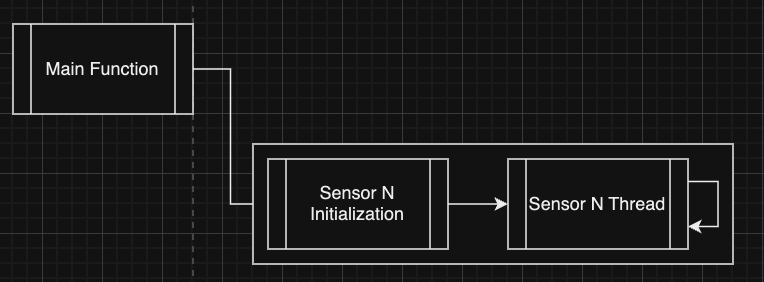
\includegraphics[width=0.8\textwidth]{images/sensor-architechure.png}
    \caption{Sensor Task Architecture}
    \label{fig:sensor-architecture} 
\end{figure} 

\subsubsection{Packet Build Tasks}
\subsubsection{Wireless Communication Tasks}
\subsubsection{Deployment Tasks}

\subsection{Middleware}

%%%%%%%%%%%%%%%%%%%%%%%%%%%%%%% Software Componets %%%%%%%%%%%%%%%%%%%%%%%%%
\chapter{Software Components}

\section{Wrappers}

\subsection{I2C Wrapper}
%%\par TODO note define CONFIG_I2C_TIMEOUT_MS = 1000
%% https://github.com/UncleRus/esp-idf-lib/tree/master/components/i2cdev


%%%%%%%%%%%%%%%%%%%%%%%%%%%%%%% Missions %%%%%%%%%%%%%%%%%%%%%%%%%
\chapter{KRUPS Aboard Norwegian GhostSat (KANG)}
\section{Kentucky Flight Computer (KFC) Requirements}

\section{FemptoSats Requirements}
\par The FemptoSats submission is to test the viability of using Wifi/LoRa for intercapsuole communication. 

\subsection{Sensors Requirements}
\par The FemptoSats will have the following sensors: 
\begin{itemize}
    \item BME280 Temperature/pressure/humidity sensor
    \item BNO086 9 - Axis IMU
\end{itemize}

\subsubsection{BME280 Temperature/pressure/humidity sensor}
\par The BME280 will be run with the following configuration settings: 

\subsubsection{BNO086 9 - Axis IMU}
\par The BNO086 will be run with the following configuration settings:

\subsection{Wireless Communcation Requirements}
\par the FemptoSat will use the following Wireless Communcation modules:
\begin{itemize}
    \item Integrated Wifi
    \item LoRa
\end{itemize}
\par The Wifi will fail over to the LoRa when the Wifi gets out of range

\section{Rocketstation Transmitter (RST) Requirements}
\par uart to raspi to shut off need

\section{Rocketstation Requirements}
\par uart to raspi to shut off need
\section{Groundstation Requirements}




%\appendix

%\newpage
%\section{Arduino Pin Mapping}
%\label{app:pinmap}
%\lstinputlisting[language={}]{arduino-pinmap.txt}

%\bibliographystyle{plain}
%\bibliography{references}
\end{document}
